% !TEX root = paper.tex
% !TEX encoding = UTF-8 Unicode
% -*- coding: UTF-8; -*-
% vim: set fenc=utf-8
% !TEX spellcheck = en-US
%=================================================================
\section{Methods}
\label{sec:methods}
%=================================================================
%=================================================================
%------------------------------%
%: see Figure~\ref{fig:methods}
\begin{figure}[t!]%%[p!]
\centering{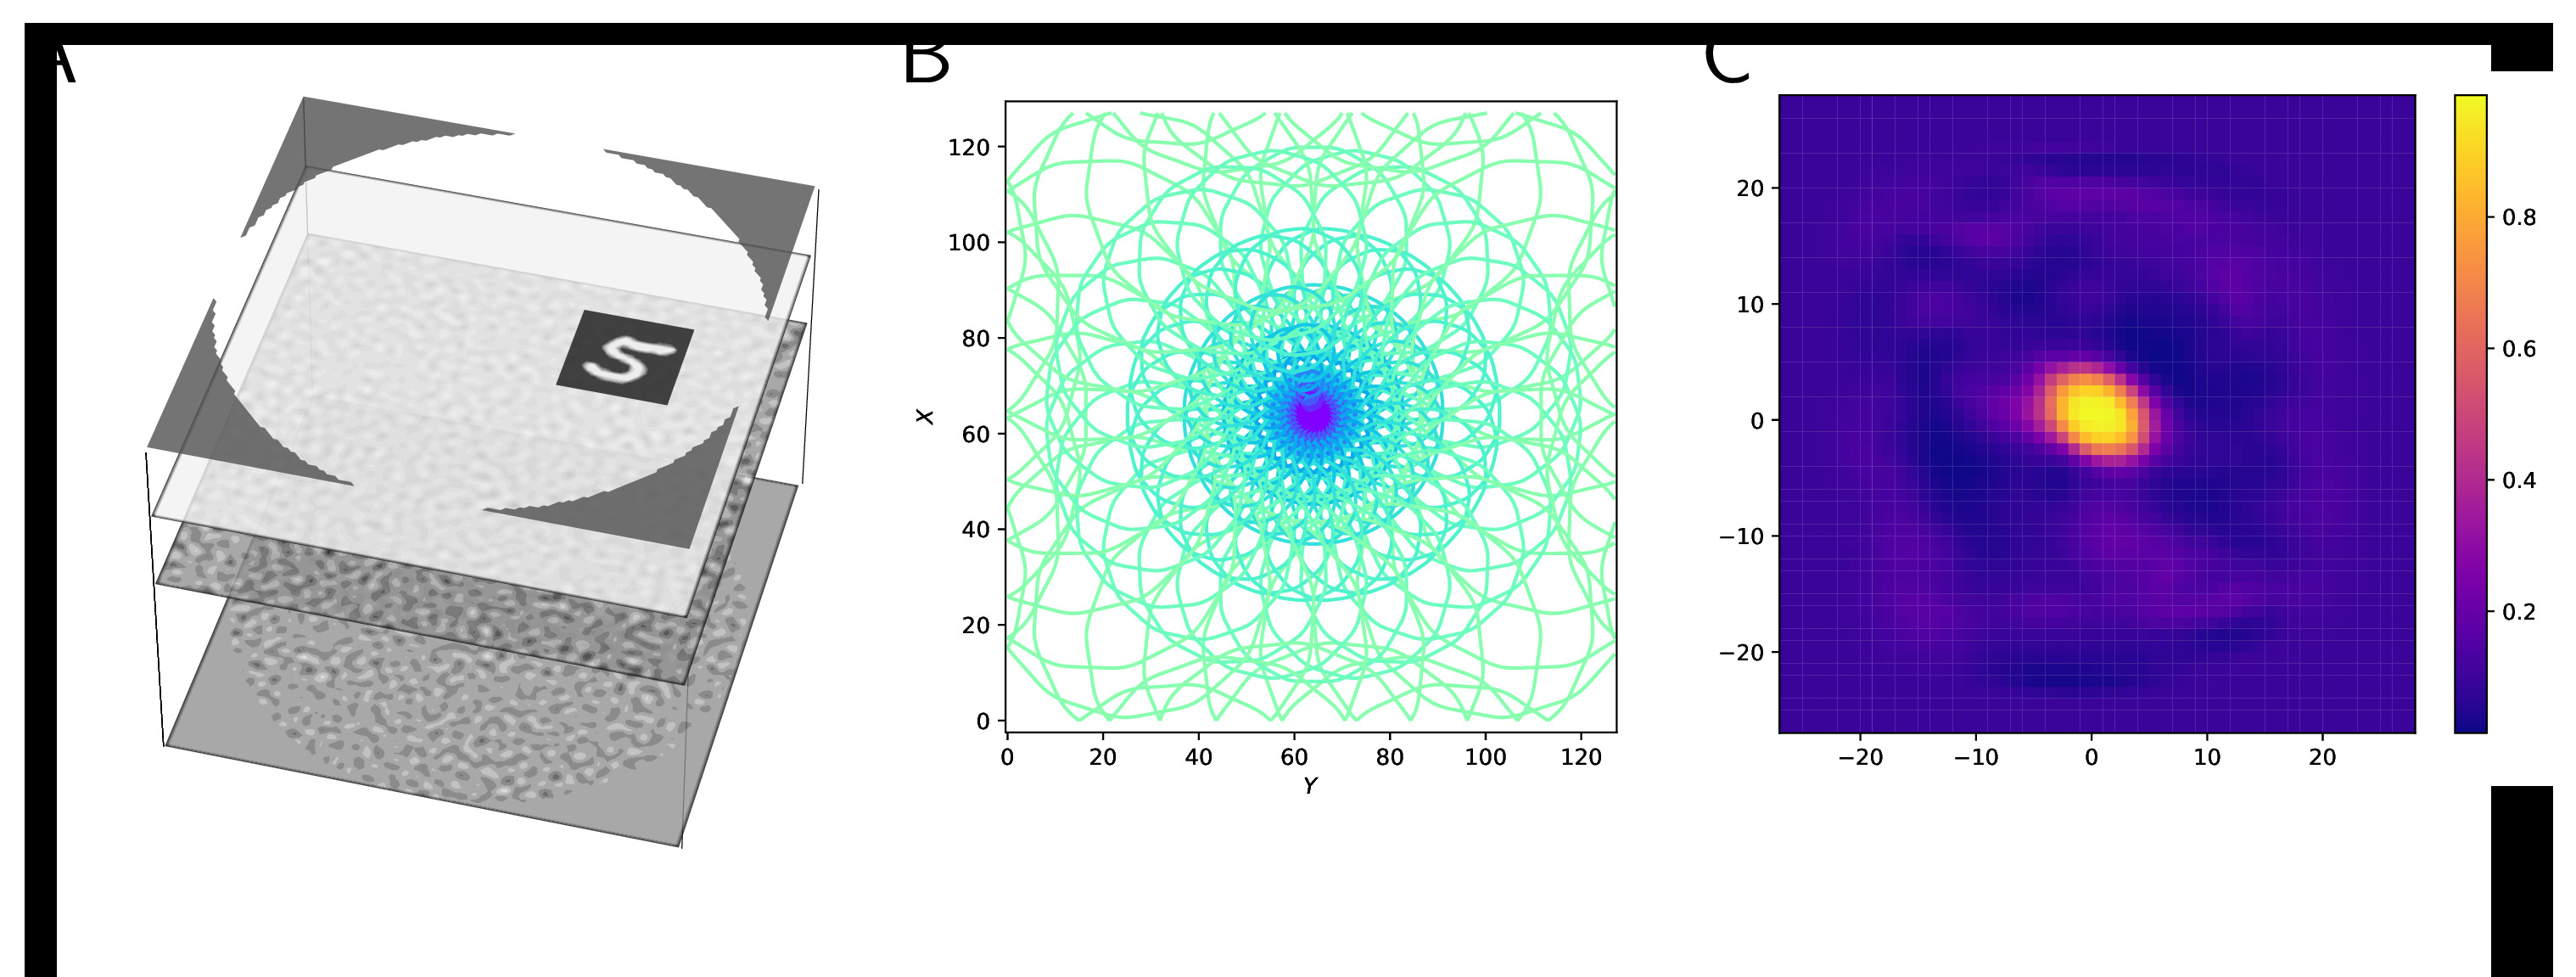
\includegraphics[width=\linewidth]{fig_methods}}
\caption{
{\bf Methods for simulating active vision}:
\A We first define the model which generates images. It is composed of three different random processes: one choosing a sample image from the MNIST database (of size $28\times 28$) and placing it at a random position within the circular mask on the $128\times 128$ display. Then, this image is rectified and multiplied by a contrast factor and finally embedded in a natural-like noise characterized by noise contrast, mean spatial frequency and bandwidth~\citep{Sanz12}. %
\B The full-sized images are transformed into a retinal image which will be fed to the ``where'' pathway. This is implemented by a bank of filters whose centers are positioned on a log-polar grid and whose radius increases proportionally with eccentricity. In addition, a similar topographic map is used to represent the accuracy of each hypothetical position of a saccade, as represented by the collicular map. %
\C The ``where'' pathway is implemented by a three-layered neural network consisting of the retinal input, two hidden layers with $1000$ units each and a collicular output. Each unit is associated with a ReLU non-linearity. To learn to associate the output of the network with the ground truth, supervised training is performed using back-propagation with a binary cross entropy loss. This scalar measures the distance between both distributions (it is always positive and null if and only if they are equal). The network learns in about $20$ epochs as shown by the decrease of the loss function. Overlaid is the associated accuracy of the full active agent. This is computed by classifying the foveal image using the ``what'' pathway, after centering the gaze using the result of the ``where pathway''. This shows a gradual increase in accuracy from the baseline ($10\%$) to approximately an average of $X80.0X\%$. %
		\label{fig:methods}}%
\end{figure}%
%%------------------------------%
In this study, the visual scene is made of a target foreground object placed at a random position over a noisy background. An agent controls a foveal visual sensor that can move over the visual scene through saccades (see Figure~\ref{fig:intro}). 
%We will define a neural network which implements this control process. 
The agent aims at understanding the visual scene, namely identifying both the target position and identity from visual samples.

\paragraph{Active inference}
Active inference assumes a hidden external state $e$, which is known indirectly through its effects on the sensor. The external state  corresponds to the physical environment. The visual field $x$ is the state of the sensors, that is a partial view of the visual scene, measured through a generative process : $x\sim p(X|e)$. The real physical state $e$ being hidden, a parametric model $\theta$ is assumed to allow estimate the cause of the current visual field through model inversion thanks to Bayes formula, in short:
$$p(E|x) \propto p(x|E;\theta)$$


The external state is assumed to split in two (independent) components, namely $e = (u,y)$ with $u$ the interoceptive body posture (in our case the gaze orientation) and $y$ the object shape (or object identity).
It is also assumed that a set of motor commands $A = \{..., a, ...\}$ (here saccades) may control the body posture, but not the object's identity, so that $y$ is invariant to $a$.

In a predictive setup, the consequence of every saccade should be analyzed through model inversion \emph{over the future observations}, that is predicting the effect of every action to choose the one that may optimize future inferences. The benefit of each action should be quantified through a certain metric (future accuracy, future posterior entropy, future variational free energy, ...), that depend on the current inference $p(U,Y|x)$. The saccade $a$ that is selected thus provides a new visual sample from the scene statistics. If well chosen, it should improve the understanding of the scene (here the target position and category). However, estimating in advance the effect of every action over the range of every possible object shapes and body postures is combinatorially hard, even in simple cases such as vision, and thus infeasible in practice.

%To infer the position of the target, we will use the fundamental hypothesis outlined in Figure~\ref{fig:intro}: The position of an object is independent from its category. 
The predictive setup necessitates in practice to restrain the generative model in order to reduce the range of possible combinations. One such restriction, known as the ``Naïve Bayes'' assumption, considers the independance of the factors that are the cause if the view.
The independence hypothesis allows considering the position $u$ and the category $y$ being independently inferred from the current visual field, i.e $p(U,Y|x) = p(U|x) p(Y|x)$. This property is strictly true in our setting and is very generic in vision for simple classes (such as digits) and simple displays (but see~\citep{Vo12} for more complex visual scene grammars). 

The independence assumption allows to separate the scene analysis in two independent tasks. A first task consists in identifying the target (namely inferring $y$ from $x$) and a second task consists in localizing the target (namely inferring $u$ from $x$). Each task is moreover assumed to be realized in parallel through distinct computational pathways, that are referred as the  
`What'' and the ``Where'' pathways by analogy with the brain\if 1\ICANN
\else  {\bf [ref needed]}. \emph{Note that %from the retinotopic projection of the visual information, 
this independence is conditional on action: both pathways should update their beliefs upon decisions made in each respective pathway {\bf (je ne comprends pas bien cette phrase?)}}\fi. However, we will here  simplify the setting by considering only one possible saccade.
\if 1\ICANN
\else
Each pathway is here assumed to rely on different sensor morphologies. By analogy with biological vision, the target identification is assumed to rely on the very central part of the retina (the fovea), that comes with higher cones density, and thus higher spatial precision. In contrast, the target localization should rely on full visual field, with peripheral regions having a lesser sensor density and a lesser sensitivity to high spatial frequencies. 

\fi
\paragraph{Metric training}
Next, the effect of a saccade is mainly to shift the visual field from one place to another. Concretely, each saccade provokes a new visual field $x'$ and a new subjective position $u'$, while the target identity $y$ remains unchanged. Examining the current visual field $x$ allows to form two hypotheses, namely $p(U|x)$ and $p(Y|x)$. It may happen, however, that the current inferences may not be accurate enough and there may be a ``better'' eye direction from which more evidence could be grabbed, i.e. it may be worth issuing a saccade so that $p(U'|x')$ and $p(Y|x')$ should be more accurate. Choosing the next saccade thus means using a model to predict how accurate $p(U'|x')$ and $p(Y|x')$ will be after the saccade realization. 

% a full sequence of operations comprises first an initial visual examination through the where and the what pathways. This .  followed by ($ii$) a decision, ($iii$) a saccade realization and ($iv$) a second visual examination that should finally ($v$) determine the category of the target.

It is worth noting that active inference needs either the current identity $y$ or the current eye direction $u$ to be readable from the present view, in order to effectively predict future inferences, through computationally intensive predictions. In detail, modeling the full sequence of operations that lead to both estimate $p(U'|x')$ and $p(Y|x')$ means predicting the future visual field $x'$ over all possible saccades, that may be tremendously costly in case of large visual fields. 

In consequence, Instead of doing predictions from a generative model, better off is to form a statistics over the (scene understanding) benefit obtained from past saccades in the same context, that is forming an \emph{accuracy map} from the current view. This is the essence of \emph{sampling-based metric prediction} we develop here. The putative effect of every saccade should be condensed in a single number, the \emph{accuracy}, that quantifies the final benefit of issuing saccade $a$ %regarding the target identity, both assuming $p(U|\boldsymbol{x})$ and $p(Y|\boldsymbol{x})$
from the current observation $x$. If $a$ is a possible saccade and $x'$ the corresponding future visual field, the result of the categorical classifier over $x'$ can either be correct (1) or incorrect (0).
If this experiment is repeated many times over many visual scenes, the probability of correctly classifying the future visual field $x'$ from $a$ forms a probability, i.e. a number between 0 and 1, that reflects the proportion of correct and incorrect classifications.
% when issuing a saccade $a$ after seeing $\boldsymbol{x}$ (the initial visual field).
It more or less corresponds to inferring the true target identity $\hat{y}$, i.e. $p(\hat{y}|x')$, including the update of the eye direction, that is a sample of the ``real'' generative process.

To sum up, a main assumption here is that instead of trying to detect the actual position of the target, it is better for the agent to estimate how accurate the categorical classifier will be after moving the eye. This forms an accuracy map that may be learned through trials and errors, by actuating saccades %after processing the visual input, 
and taking the final classification success or failure as a teaching signal.
Such a \emph{predictive accuracy map} is assumed to be the core of a realistic saccade-based vision system.

Note that compared to a brute force approach which would scan for all possible positions in an image, this map should compress the information, as exemplified by a retinotopic map. The map should be mostly organized radially, preserving the initial retinotopic organization. %with high predicted accuracies reflecting a high probability of target presence at given locations.
The operations that transform the initial primary visual data should thus preserve the initial spatial compression, so as to form the final  retinotopic accuracy map. Accordingly with the initial data, the retinotopic accuracy map may thus provide more detailed accuracy predictions in the center, and coarser accuracy predictions in the periphery. 
%and telling how accurate the categorical classifier will be after the saccade is carried out~\citep{Dauce18}. %The set of all possible saccade predictions should

Finally, each different initial visual field may come with a different accuracy map, indirectly conveying information about the target retinotopic position. 
A final action selection (motor map) should then overlay the accuracy map through a winner-takes-all mechanism, implementing the saccade selection in biologically plausible way, as it is thought to be done in the superior colliculus\if 1\ICANN .
\else {\bf [ref needed]}.

\paragraph{Information gain and the inhibition of return}
From the information theory standpoint, each saccade comes with fresh visual information about the visual scene that can be quantified by an \emph{information gain}, namely:
\begin{align}
\text{IG}_\text{max} &= \max_{u'} \log p(y|u',x',x, u) - \log p(y|x, u)\\
          &\simeq \max_{u'} \log p(y|x') - \log p(y|x)
\end{align}
with the left term representing the future accuracy (after the saccade is realized) and the right term representing the current accuracy as it is obtained from the 'what' pathway. The accuracy gain may be averaged over many saccades and many initial eccentricities (so that the information gain may be close to zero when the initial $u$ is very central). 

For the saccade is subject to predictions errors and execution noise, the actual $u'$ may be different from the initial prediction. The final accuracy, as instantiated in the accuracy map, contains this intrinsic imprecision, and is thus necessary lower than the optimal one. The consequence is that in some cases, the approximate information gain may become negative, when the future accuracy is actually lower than the current one. This is for instance the case when the target is centered on the fovea.  This should encourage the agent to select a saccade ``away'' from the central position, which is reminiscent of a well-known phenomenon in vision known as the ``inhibition of return''~\citep{Itti01}. Combining accuracy predictions from each pathway may thus allow to refine saccades selection in a way that complies with biological vision.   

%Our main argument is that such an accuracy map is trainable in a rather straightforward way, 

\fi
To test the validity of our hypothesis, let us find a %it is necessary to find at least one 
function implementing the ``where'' network. This function should be able to find the position of an object knowing only the degraded retinal image. Here, we describe the methods that we will follow to find that function, from the generative models (first external and then internal) to the actual implementation of the ``where'' pathway. %

%Second, we %start as in~\citep{Friston12} by a probabilistic formulation, and


%
\subsection{Exteroceptive Generative model}
%=================================================================
We define here the generative model for input display images as shown first in Figure~\ref{fig:intro}-A (\DIS ) and as implemented in Figure~\ref{fig:methods}-A.

\paragraph{Targets.} Following a common hypothesis regarding active vision, visual scenes consist of a single visual object of interest. We use the MNIST database of handwritten digits introduced by~\citep{Lecun1998}. %Indeed, we are here focused on the problem of localization (``where'' pathway) and classification solutions (``what'' pathway) abound for this class of targets. 
Samples are drawn from a database of $60000$ grayscale $28\times 28$ pixels images and separated between a training and a validation set (see below the description of the ``where'' network).

\paragraph{Full-scale images.} Each sample position is draw a random in a full-scale image of size $128\times 128$. To enforce isotropic saccades, a centered circular mask covering the image (of radius $64$ pixels) is defined, and the position is such that the embedded sample fits entirely into that circular mask.

\paragraph{Background noise setting. } To implement a realistic background noise, we generate synthetic textures~\citep{Sanz12} using a bi-dimensional random process. %The generated texture images are of the same size than the full-image. 
The texture is designed to fit well with the statistics of natural images. We chose an isotropic setting where textures are characterized by solely two parameters, one controlling the median spatial frequency $sf_0$ of the noise, the other controlling the bandwidth around the central frequency. Equivalently, this can be considered as the band-pass filtering of a random white noise image. Finally, these images are rectified to have a normalized contrast.

\paragraph{Mixing the signal and the noise. } Finally, both the noise and the target image are merged into a single image. Two different strategies are used. A first strategy emulates a transparent association, with an average luminance computed at each pixel, while a second strategy emulates an opaque association, choosing for each pixel the maximal value. The quantitative difference was tested in simulations, but proved to have a marginal importance.
%
\subsection{Interoceptive generative model}
%=================================================================
%
We  now define the simplified anatomy of the agent, which is composed of two separate pathways.

\paragraph{Foveal vision and the ``what'' pathway}
First, foveal vision is defined as the $28\times 28$ pixels image centered at the point of fixation (see dashed red box in Figure~\ref{fig:intro}-C). This image is then directly passed to the agent's visual categorical pathway (the ``What'' pathway). This is realized by the known ``LeNet'' classifier~\citep{Lecun1998}, that processes the $28 \times 28$ central pixels to identify the target category. Such a network is directly provided (and unmodified) by the pyTorch library~\citep{Paszke17}, and consists of a 3-layered Convolutional Neural Network. It is trained over the (centered) MNIST database after approx $20$ training epochs. \if 1\ICANN
\else
Input images are rectified (\emph{with a mean and standard deviation of respectively $0.1307$ and $0.3081$ {\bf why??}}). \fi The network outputs a vector representing the probability of detecting each of the $10$ digits. We use the argument of the output neuron with maximum probability, to categorize each image. This strategy achieves an average $98.7\%$ accuracy on the validation dataset~\citep{Lecun1998}. %

\paragraph{Retinal transform: Peripheral vision and log Polar encoding}
First, both the visual features and the expected target position may to be expressed in retinal coordinates which we choose here to be log-polar as it provides a good fit with observations in mammals~\citep{Traver10}. On the visual side, we extracted local visual features as oriented edges  as the combination of the retinotopic transform with that of the primary visual cortex~\citep{Fischer2007a}. The centers of these first and second order orientation filters are radially organized around the center of fixation, with small and tightened receptive fields at the center and more large and scarce receptive fields at the periphery, see  Figure~\ref{fig:methods}-B. The size of the filters increases proportionally to eccentricity. The filters are organized in $10$ spatial eccentricity scales (respectively placed at around $2$, $3$, $4.5$, $6.5$, $9$, $13$, $18$, $26$, $36.5$ , and $51.3$ pixels from the center) and $16$ different azimuth angles allowing them to cover most of the original $128 \times 128 $ image. At each of these position, we computed $10$ different edge orientations and $2$ different phases (symmetric and anti-symmetric) using log-Gabor filters~\citep{Fischer2007a}. This finally implements a (fixed) bank of linear filters which model the receptive fields of the input to the primary visual cortex.

From any input image ($128\times 128=16384$ pixels) is linearly transformed into a retinal activity vector $\boldsymbol{x}$. Note that to ensure balace of the coefficients across scales, the images are first whitened. In practice, the length of this vector is $1600$ such that the retinal filter compresses the original image by about 90\%, with high spatial frequencies preserved at the center and only low spatial frequencies conserved at the periphery. In practice, this filters are pre-computed and placed into a matrix for a rapid transform of batches of input displays into retinal transforms. In practice this matrix transformation allows also the evaluation of a reconstructed visual image given a retinal activity vector thanks to the pseudo-inverse matrix of the forward transform matrix. In summary, the full-sized images are transformed into a peripheral retinal image which will be fed to the ``where'' pathway.

\paragraph{Collicular representation: accuracy map}
We will now define the output of the ``Where'' pathway as an \emph{accuracy map} representing the probability of the presence of a target in the visual field, independently of its identity. As the retinotopic map, this target accuracy map is also organized radially in a log-polar fashion, making the target position estimate more precise at the center and fuzzier at the periphery. This modeling choice is reminiscent of the approximate log-polar organization of the superior colliculus (SC) motor map. In ecological conditions, the accuracy map is trained by sampling, i.e. by "trial and error", using for instance corrective saccades to compute (a posteriori) the probability of a correct localization. In a computer simulation however, this induces a combinatorial explosion which does render the calculation not amenable.

However, as we generated the display, we know the position of the target (which is hidden to the agent). Moreover, we observed that we could also evaluate the accuracy of the classifier (that is the fixed ``what'' pathway) knowing the translational shift imposed to the input foveal image by a saccade of known amplitude. Knowing the size of the $28\times 28$ input image, this generates a $55\times 55$ accuracy map (larger shift correspond to a target outside the fovea and necessary an accuracy at the chance level of $10\%$). This classifier displays a high accuracy at the center (with a value of $98.7\%$ corresponding to the validation score without any translational shift), and a fast decreasing accuracy with target eccentricity, as shown in Figure~\ref{fig:results}-D. By assuming ergodicity, knowing this centered accuracy map, this allows us to rapidly predict for each visual display the full accuracy map at each pixel by shifting the centered accuracy map on the true position of the target. Such a computational shortcut is allowed by the independence of the categorical performance with position thanks to the independence which is implemented in the exteroceptive generative model.

Finally, we will project this full accuracy map on the collicular map to compute the accuracy of each hypothetical saccade in the collicular space (see  Figure~\ref{fig:methods}-B, "True"). In practice, we will use the energy of the filters at each position as a proxy to quantify the projection from the visual space of the display to the collicular space. This generates a filter bank at $10$ spatial eccentricity scales and $16$ different azimuth angles, and $160$ collicular receptive fields. Each filter is normalized such that the value at each collicular position is the average of the values which are integrated in visual space. Applied to the full sized ground truth accuracy map computed in display space, this gives an accuracy map at different location of motor space. Such collicular transform is again implemented by a simple matrix multiplication which can be pre-computed and particularly is rapid to compute. Practically, this also allows to compute an inverse transform using the pseudo-inverse matrix of the forward transform. In particular, we will use that inverse transform to represent the accuracy predicted by any given collicular vector, but also to compute the position in display space of maximal accuracy.

\subsection{Implementing the ``where'' pathway}
%=================================================================


\paragraph{Classifier training using deep learning}
Modern parametric classifiers are composed of many layers (hence the term ``Deep Learning'') that can be trained through gradient descent over arbitrary input and output feature spaces. The ease of use of those tightly optimized training algorithms allow to quantify the difficulty of a task through the failure or success of such training. Consider the retinal transform $\boldsymbol{x}$ as the input and a log-polar retinotopic vector $\boldsymbol{a}$ made of $n$ Bernouilli probabilities (success probabilities) as the output. Following the active inference framework, we will train the network to predict the distribution $\boldsymbol{a}$ knowing the retinal input $\boldsymbol{x}$ by comparing it to the known ground truth distribution computed over the collicular map. As a loss function, we will naturally use the Kullback-Leibler divergence between the ground truth and the predicted map.

%The ``What'' pathway will be given from the literature. In contrast, the ``Where'' pathway takes the into account in order to tell whether a target is present at the different peripheral locations, in order to monitor future saccades. 


In practice, the parametric neural network is made of an input (retinal) layer, two fully connected hidden layers of size $500$ and $2000$ units respectively and an output layer, with ReLu activation between each layer, except at the output which uses a sigmoid function to ensure that the output is compatible with the representation of a likelihood. In addition, we tested the effect of $50 \%$ drop-out on the last hidden layer. Another improvement in convergence speed was obtained by using Batch normalization. The network is trained over $500,000$ saccades on full-images, using the binary cross-entropy loss as the error signal, with a learning rate equal to $10^{-4}$ and stochastic gradient descent with a momentum to improve convergence. The training is done for $25$ epochs in about $1$ hours on a laptop. The code is written in Python (version 3.7.6) with pyTorch library~\citep{Paszke17} (version 1.0.1). The full scripts for reproducing the figures and extending the results to a full range of parameters is available at \url{https://github.com/laurentperrinet/WhereIsMyMNIST}. % TODO: change to https://github.com/SpikeAI/DauceAlbigesPerrinet19 when public 
